% ============================ Enrico Ribiani 16-03-2021 ====================================================================
% Base per i documenti  
\documentclass[12pt]{article}
% ------------ pacchetti necessari ----------------
\usepackage[a4paper, total={6in, 8in},margin=1in]{geometry} % formattazione decente della pagina
\usepackage{graphicx}                            % need for figure
\usepackage{amsmath}
\usepackage{amsfonts}                            % if you want the fonts
\usepackage{amssymb}                             % if you want extra symbols
\usepackage{graphicx}  
\renewcommand{\figurename}{Figura}  
\renewcommand{\contentsname}{Indice}                        % need for figures
\usepackage{mathptmx}
\usepackage{float}                               % serve per mettere tabelle e immagini dove si vuole 
\usepackage[utf8]{inputenc}
\usepackage{textcomp}
\usepackage[hang,flushmargin,bottom]{footmisc}   % footnote format
\usepackage{fancyhdr, lastpage}
\usepackage{titlesec}
\usepackage[table,dvipsnames]{xcolor}
%\pagestyle{fancy}
%\renewcommand{\headrulewidth}{0pt}
%\renewcommand*\contentsname{Indice}
\titleformat{\section}{\normalsize\bfseries}{\thesection.}{1em}{}	% required for heading numbering style
\titleformat*{\section}{\Large\bfseries}
\titleformat*{\subsection}{\large\bfseries}
%\usepackage{siunitx}
%\usepackage{tikz}
\usepackage{circuitikz}
%\usepackage[siunitx]{circuitikz}
\usepackage{multirow}
\usepackage{tikz}
\usepackage{amsmath}
\usetikzlibrary{angles,quotes}
\usepackage{placeins}
\usepackage{multirow}
%===================links=================
\usepackage{hyperref}
\hypersetup{
    colorlinks=true,
    linkcolor=Sepia,
    filecolor=Green,      
    urlcolor=Cyan,
    pdftitle={SAMPLE},
    pdfpagemode=FullScreen,
    }
    \usepackage{kvoptions}
    \usepackage{xcolor-material}
    \definecolor{nred}{RGB}{191, 97, 106}
    \definecolor{norange}{RGB}{208, 135, 112}
    \definecolor{nyellow}{RGB}{163, 190, 140}
    \definecolor{ngreen}{RGB}{35, 203, 139}
    \usepackage{colortbl}
    \usepackage{nicematrix}
%===================inizio pagina del titolo=================
\begin{document}
    \begin{titlepage}
    \begin{center}
% ------------------ inizio immagine logo ----------
\begin{figure}
    \centering
    
\includegraphics{~/varie/logo.png}
    \label{fig:logo}
\end{figure}
% ------------------ fine immagine logo ----------
% ------------------ fine immagine logo ----------
-------------------------------------------------------------------------------------\\
\vspace{2\baselineskip}
\large Enrico Ribiani\\
\large 4AUB\\
\vfill

\Huge{\textbf{Esperienza laboratoriale bipolo ohmico-capacitivo-induttivo serie}}\\
\vfill

\LARGE{esperienza n°2}\\
\vfill
\large{19-10-2021}
\end{center}
%=============== fine pagina titolo ===============
\end{titlepage}
\tableofcontents
\vskip 1cm
\section{Scopo:Verificare il comportamento di un bipolo sperimentalmente confrontanto i valori reali con quelli teorici.}
    \subsection{Materiale}
    \begin{itemize}
        \item Breadboard
        \item Condensatore da \textit{100nF}
        \item Resistenza da \textit{2,2k$\Omega$}
        \item Induttore da \textit{47mH}
    \end{itemize}
    \subsection{Strumenti}
    \begin{itemize}
        \item Generatore di funzione
        \item Oscilloscopio
        \item Multimetro
    \end{itemize}
        \subsubsection{Schema}
        
        \begin{center}
            Il primo circuito verrà utilizzato per effettuare le misure su R, il secondo per effettuare le misure su C e il terzo per le misure su L.
        \end{center}
        \vskip 1cm
        \begin{circuitikz}[american voltages]
            \draw
                (0,0) -- (0,-0.2) node[ground]{}    
                to[vsourcesin, l_=\textit{v(t)}] (0,4)
                (0,4) to [short, *-, l=Ch1] (0,4)
                to[american resistor,  l_=R \textit{2,2k$\Omega$}, i=\textit{i(t)}] (4,4) 
                (4,4) to [inductor, *-, l=L \textit{47mH}] (4,0) %label ch2 da fixare
                to[capacitor, l=C\textit{100nF}] (0,0)
                (0,0) to [short, *-] (0,0)
                
            ;
        \end{circuitikz}
       
        \vskip 1cm

   \begin{circuitikz}[american voltages]
    \draw
        (0,0) -- (0,-0.2) node[ground]{}    
        to[vsourcesin, l_=\textit{v(t)}] (0,4)
        (0,4) to [short, *-, l=Ch1] (0,4)
        to[capacitor, l=C \textit{100nF}] (4,4) 
        (4,4) to [inductor, *-, l=L \textit{47mH}] (4,0) %label ch2 da fixare
        to[american resistor,  l_=R \textit{2,2k$\Omega$}] (0,0)
        (0,0) to [short, *-] (0,0)
    ;
\end{circuitikz}

\vskip 1cm

\begin{circuitikz}[american voltages]
 \draw
     (0,0) -- (0,-0.2) node[ground]{}    
     to[vsourcesin, l_=\textit{v(t)}] (0,4)
     (0,4) to [short, *-, l=Ch1] (0,4)
     to [inductor, *-, l=L \textit{47mH}] (4,4) 
     (4,4) to[capacitor, *-, l=C \textit{100nF}] (4,0) 
     to[american resistor,  l_=R \textit{2,2k$\Omega$}] (0,0)
     (0,0) to [short, *-] (0,0)
 ;
\end{circuitikz}


\section{Cenni teorici}
    %\subsection*{Generalità bipolo RLC}
   
    \subsection{Previsione comportamento}
    Il bipolo RLC è un circuito formato da un induttore, un resistore e un capacitore che in un aregime alternato si 
    comporta diversamente al variare della frequenza dal momento che $X_L$ e $X_C$ ne dipendono, ci sono tre scenari possibili:
    \begin{enumerate}
        \item $X_C>X_L$\\
        In questo caso il bipolo si comporterà come un bipolo RC quindi la tensione $\vec{V}$ sarà in ritardo di 90° rispetto alla corrente $\vec{I}$
        \item $X_L>X_C$\\
        In questo caso il bipolo si comporterà come un bipolo RL quindi la tensione $\vec{V}$ sarà in anticipo di 90° rispetto alla corrente $\vec{I}$
        \item $X_L$=$X_C$\\
        In questo caso il bipolo si comporterà come un bipolo puramente resistivo quindi $\vec{V}$ sarà in fase con $\vec{I}$ in quanto la parte immaginaria del 
        vettore sarà completamente nulla.
        
    \end{enumerate}
    In questa esperienza osserveremo sperimentalmente tutti i tre casi utilizzando tre diverse frequenze, mi aspetto che 
    le sinusoidi si comportnordicino in base alla frequenza come scritto precendentemente a meno di piccole variazioni dovuti agli srumenti di 
    misura e a i vari errori.
\section{Procedimento}
   Dopo aver controllato il materiale,calcolato fr, misurato R e $R_{pind}$ che è la resistenza parassita dell'induttore abbiamo collegato il circuito al generatore
   di funzione e l'oscilloscopio, con un circuito montato abbiamo eseguito le misurazioni per tutte le frequenze prima su R, poi abbiamo collegato l'oscilloscopio ai capi
   di C e abbiamo preso le misure per tute le frequenze, idem per L.\\
   Mentre cambiavamo frequenza dal generatore d'onda abbiamo scritto le misure sulla tabella e fatto le foto dell'oscilloscopio.
   una volta misurato il valore di tensione e tempo di ritardo \textit{$t_r$} abbiamo calcolato lo sfasamento. 
   
   \vskip 1cm 
   \subsection{Foto}
    \begin{figure}[!h]
        \centering
        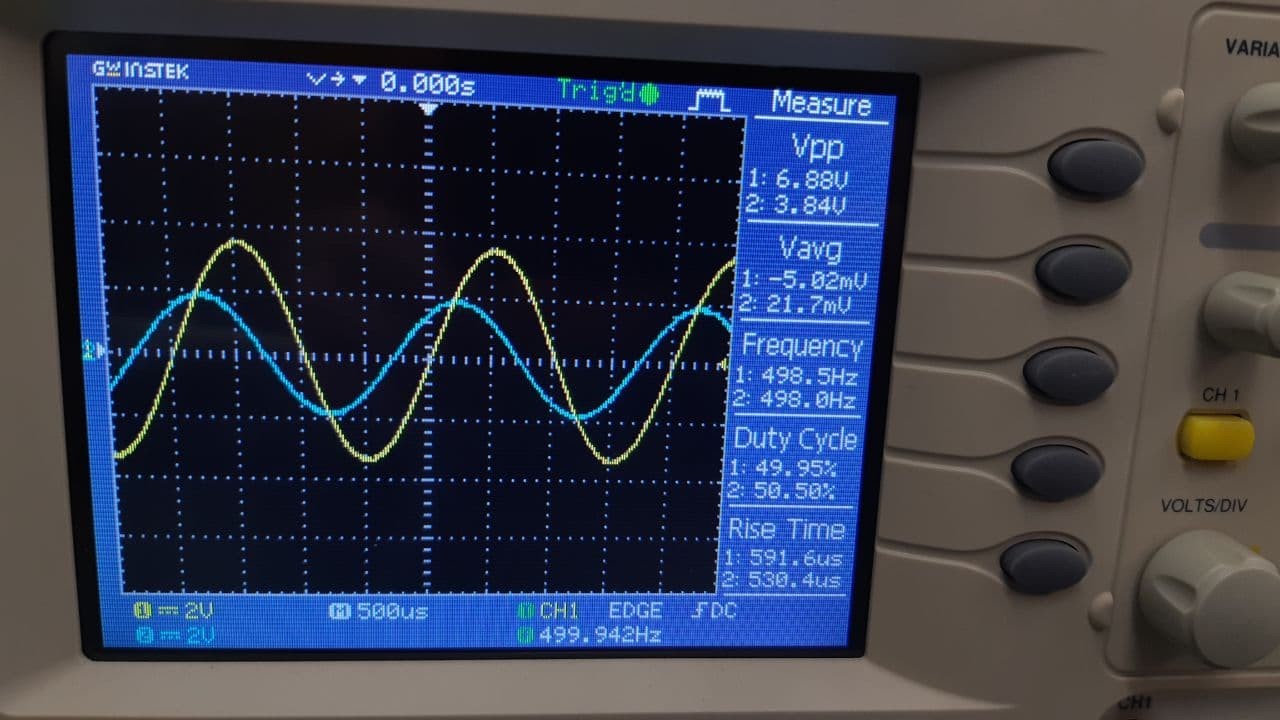
\includegraphics[scale=0.2]{media/f1vr.jpg}
        \caption{$V_R$ 500Hz}
    \end{figure}
    \begin{figure}[!h]
        \centering
        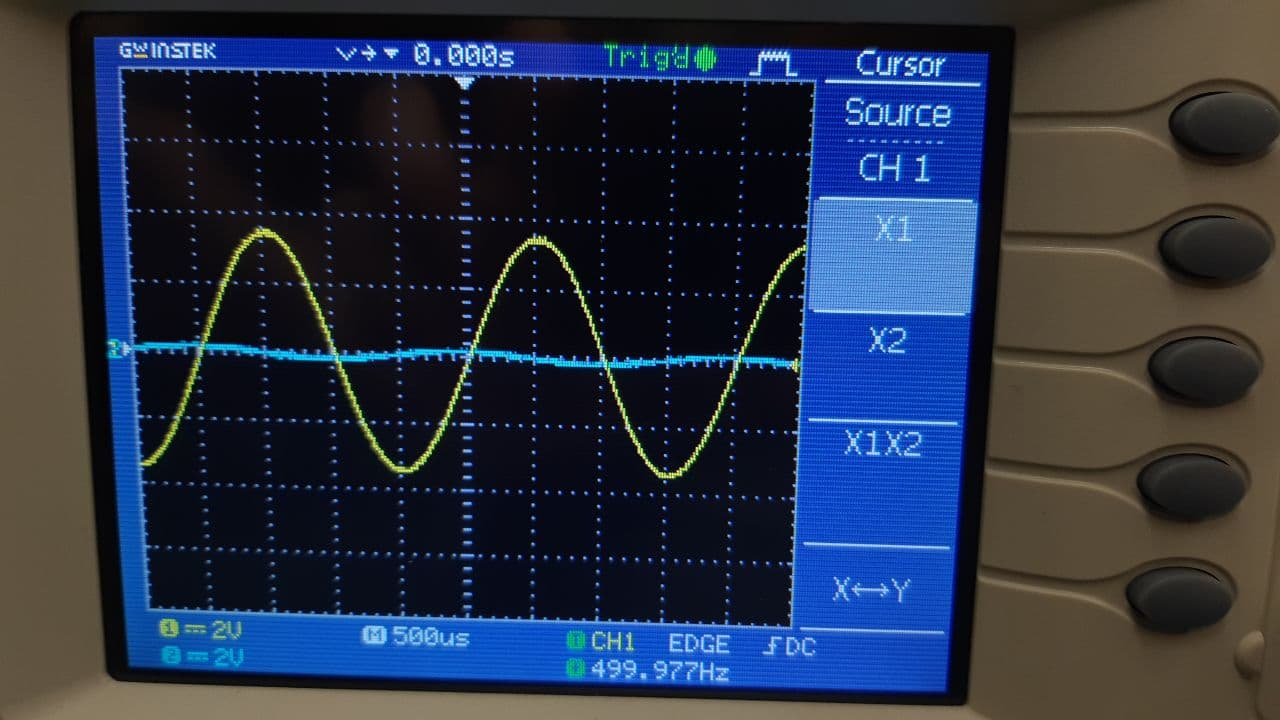
\includegraphics[scale=0.2]{media/f1vl.jpg}
        \caption{$V_L$ 500Hz}
    \end{figure}
    \begin{figure}[!h]
        \centering
        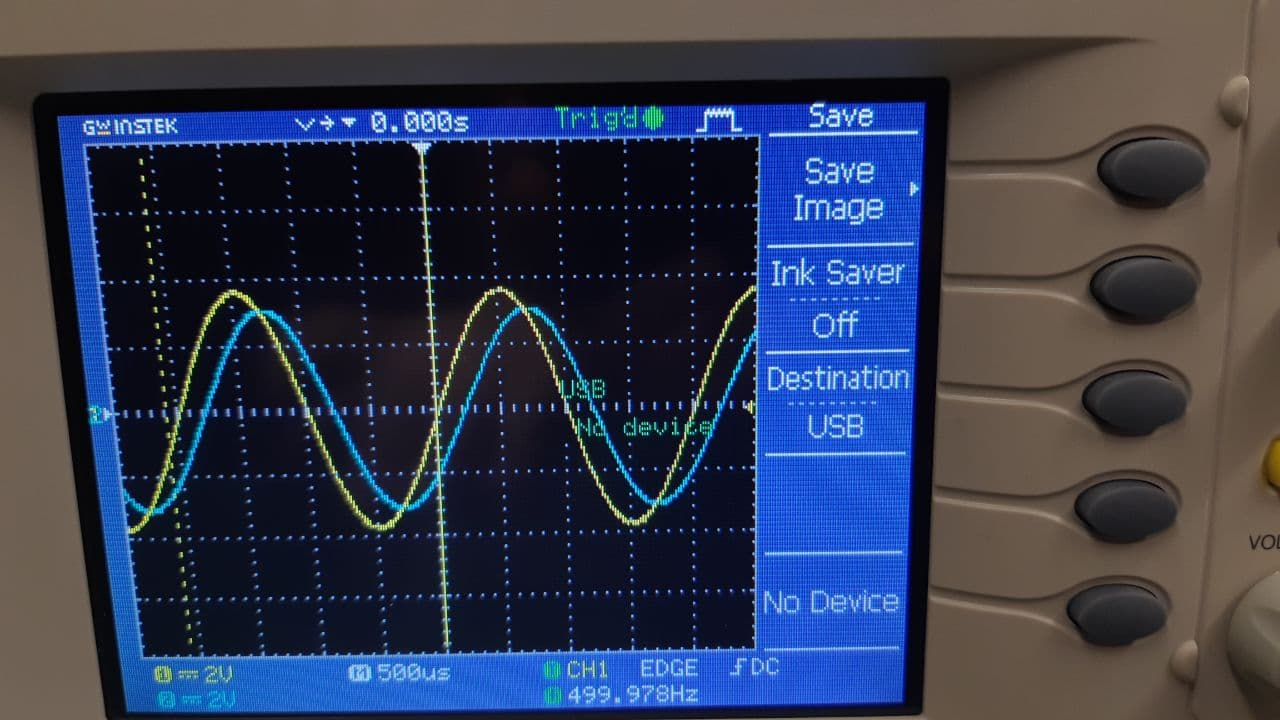
\includegraphics[scale=0.2]{media/f1vc.jpg}
        \caption{$V_C$ 500Hz}
    \end{figure}
    \begin{figure}[!h]
        \centering
        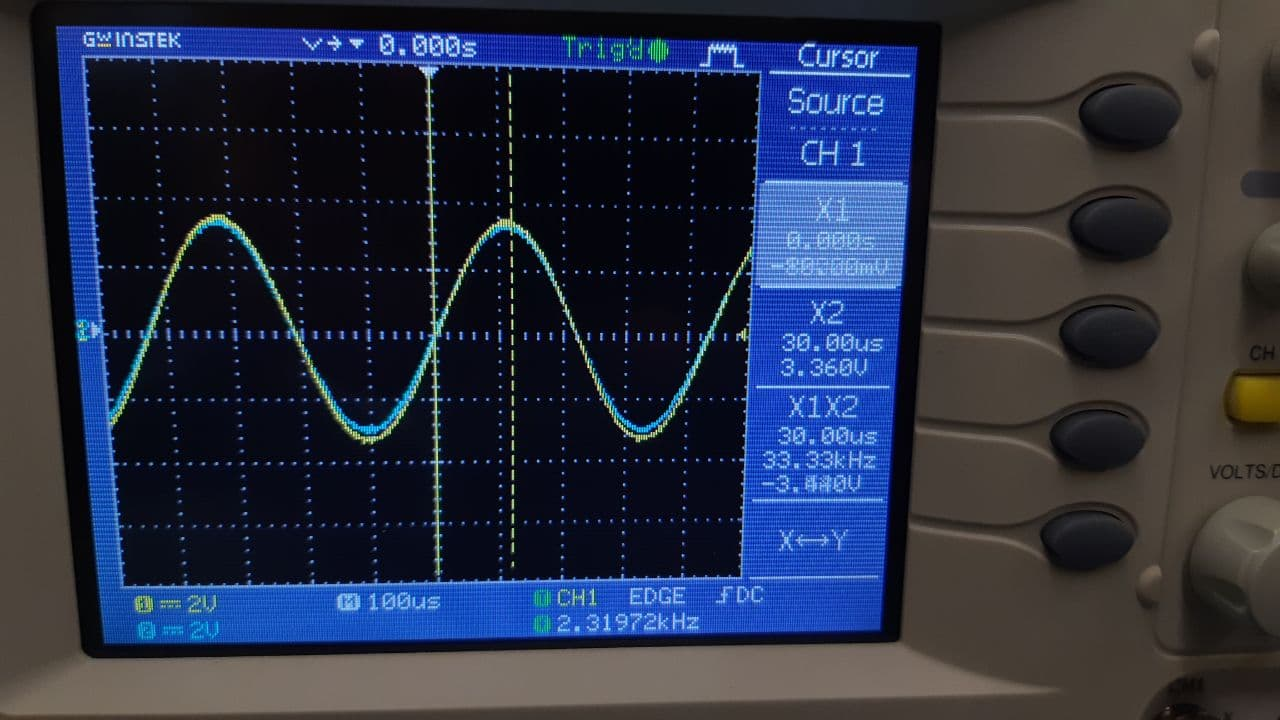
\includegraphics[scale=0.2]{media/frvr.jpg}
        \caption{$V_R$ fr}
    \end{figure}
    \begin{figure}[!h]
        \centering
        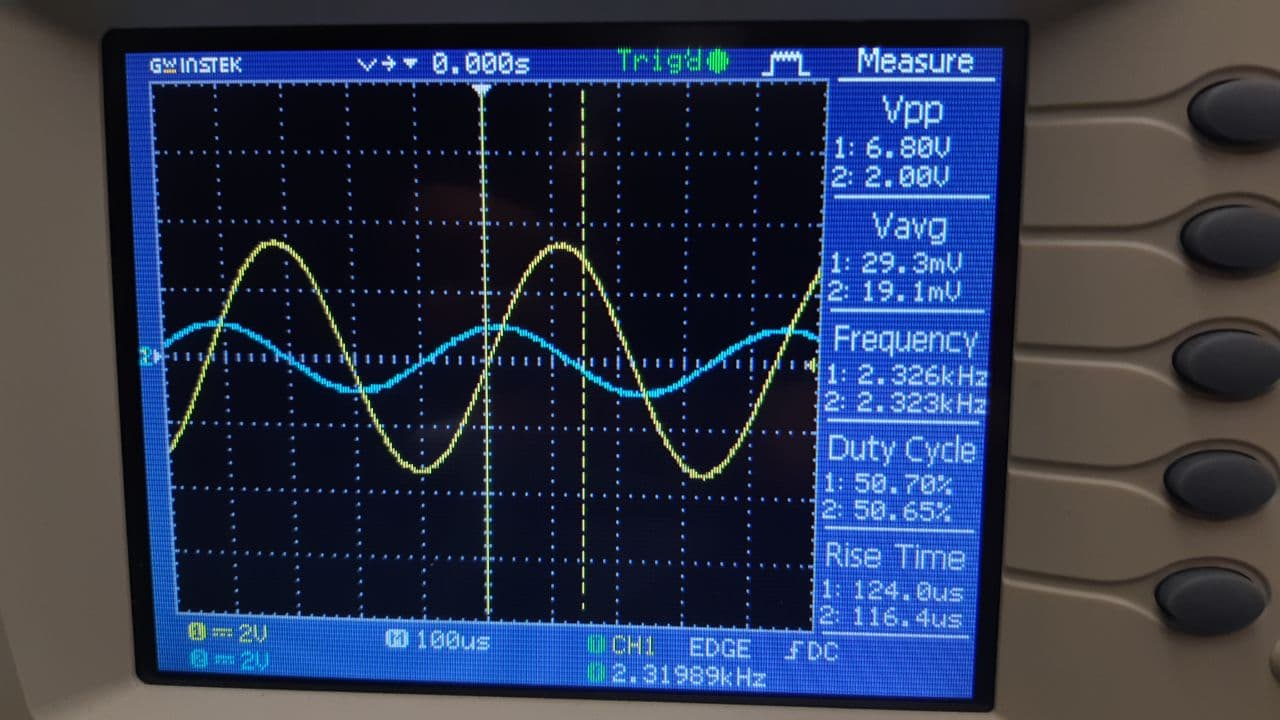
\includegraphics[scale=0.2]{media/frvl.jpg}
        \caption{$V_L$ fr}
    \end{figure}
    \begin{figure}[!h]
        \centering
        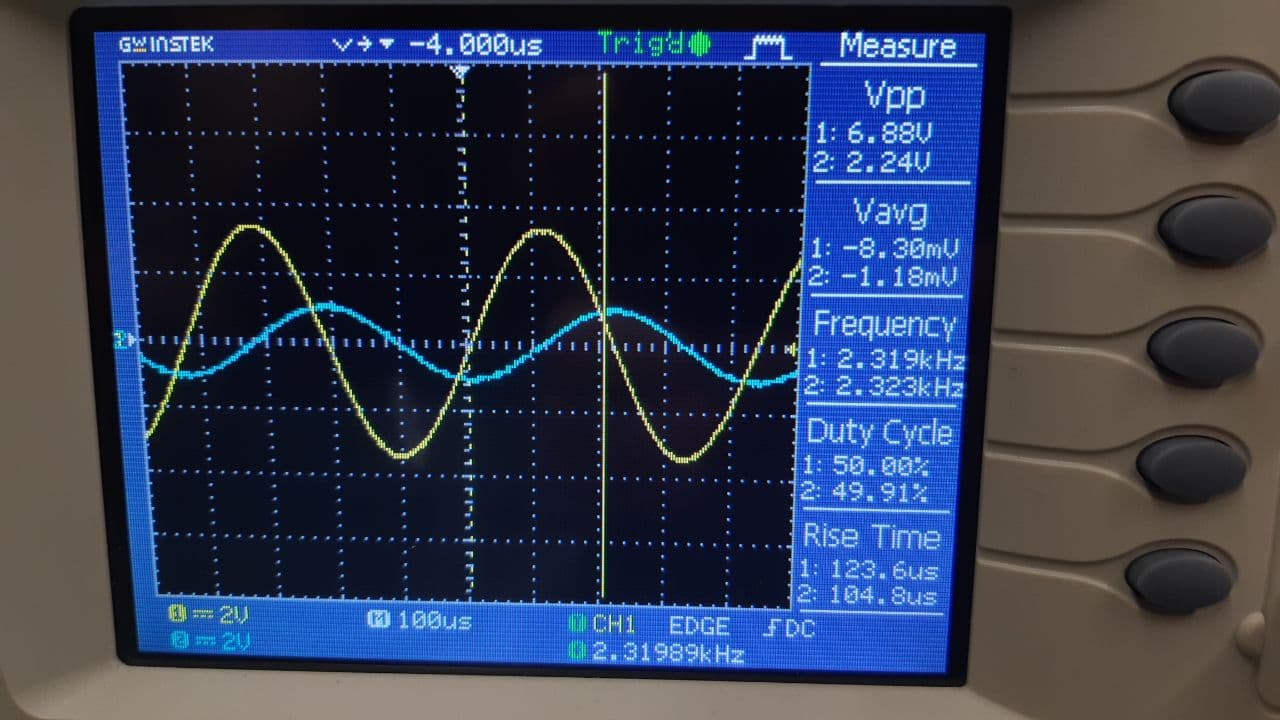
\includegraphics[scale=0.2]{media/frvc.jpg}
        \caption{$V_C$ fr}
    \end{figure}
    \begin{figure}[!h]
        \centering
        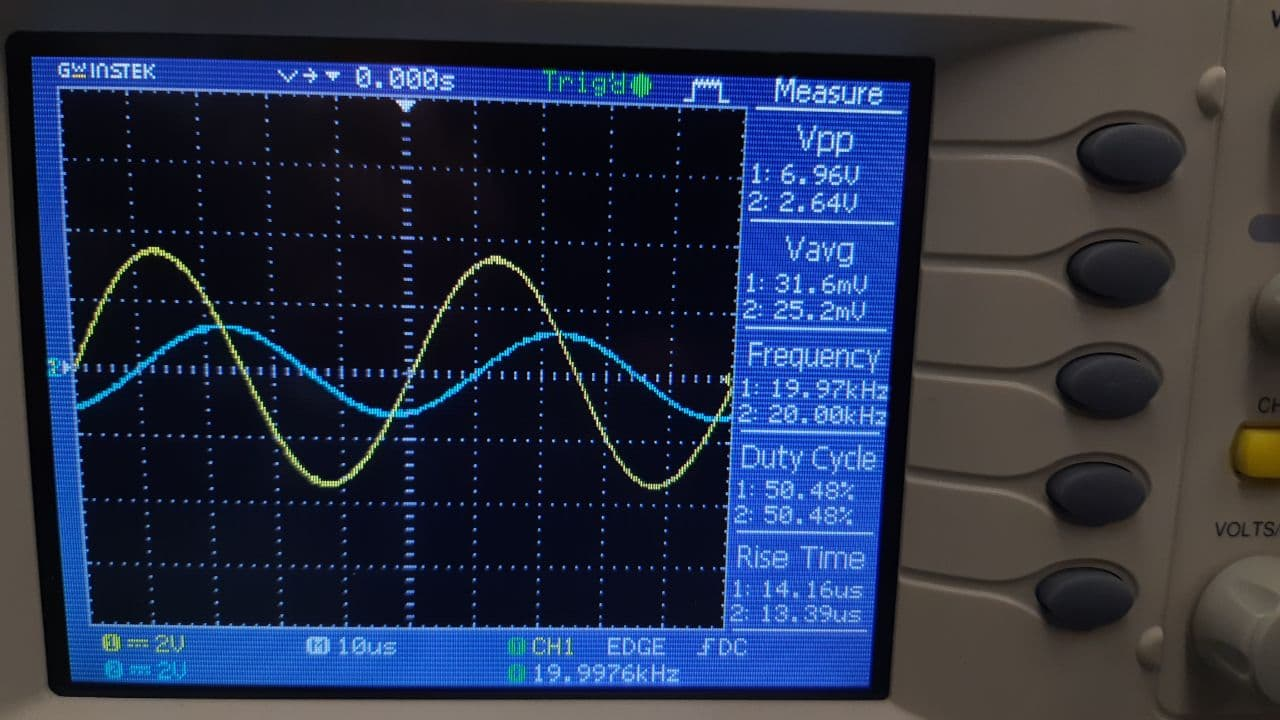
\includegraphics[scale=0.2]{media/f2vr.jpg}
        \caption{$V_R$ f=20kHz}
    \end{figure}
    \begin{figure}[!h]
        \centering
        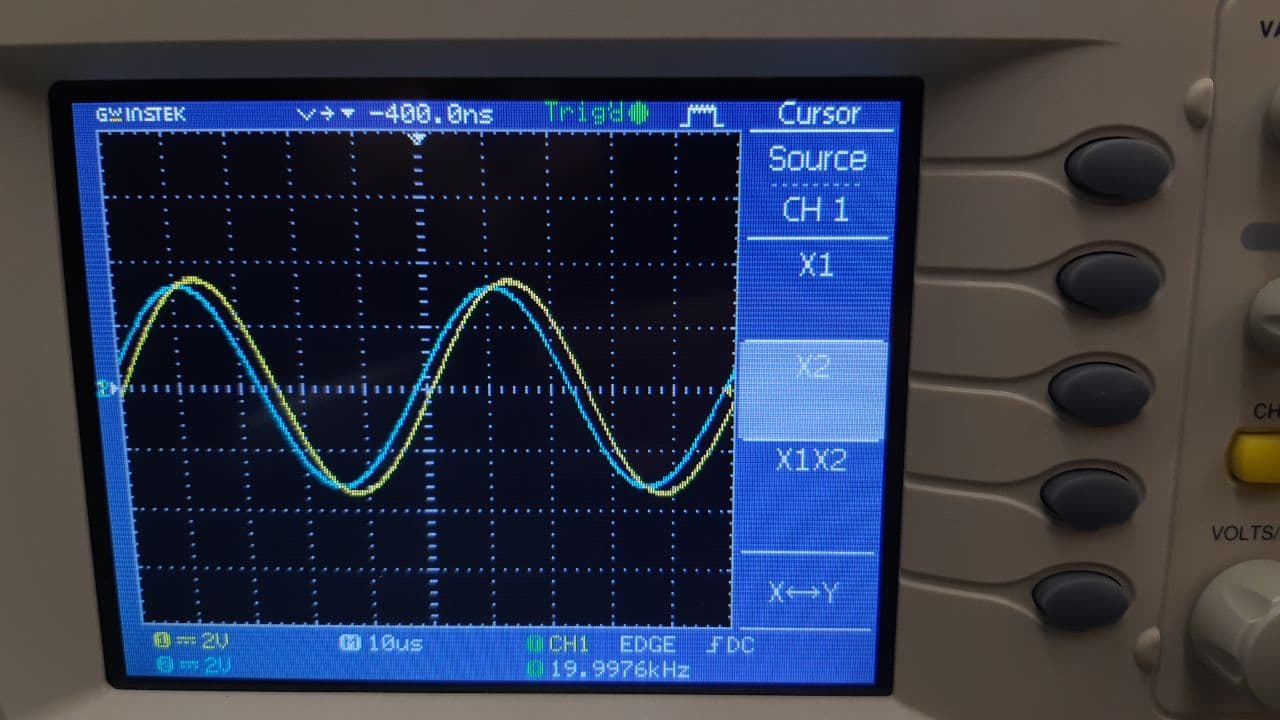
\includegraphics[scale=0.2]{media/f2vl.jpg}
        \caption{$V_L$ f=20kHz}
    \end{figure}
    \begin{figure}[!h]
        \centering
        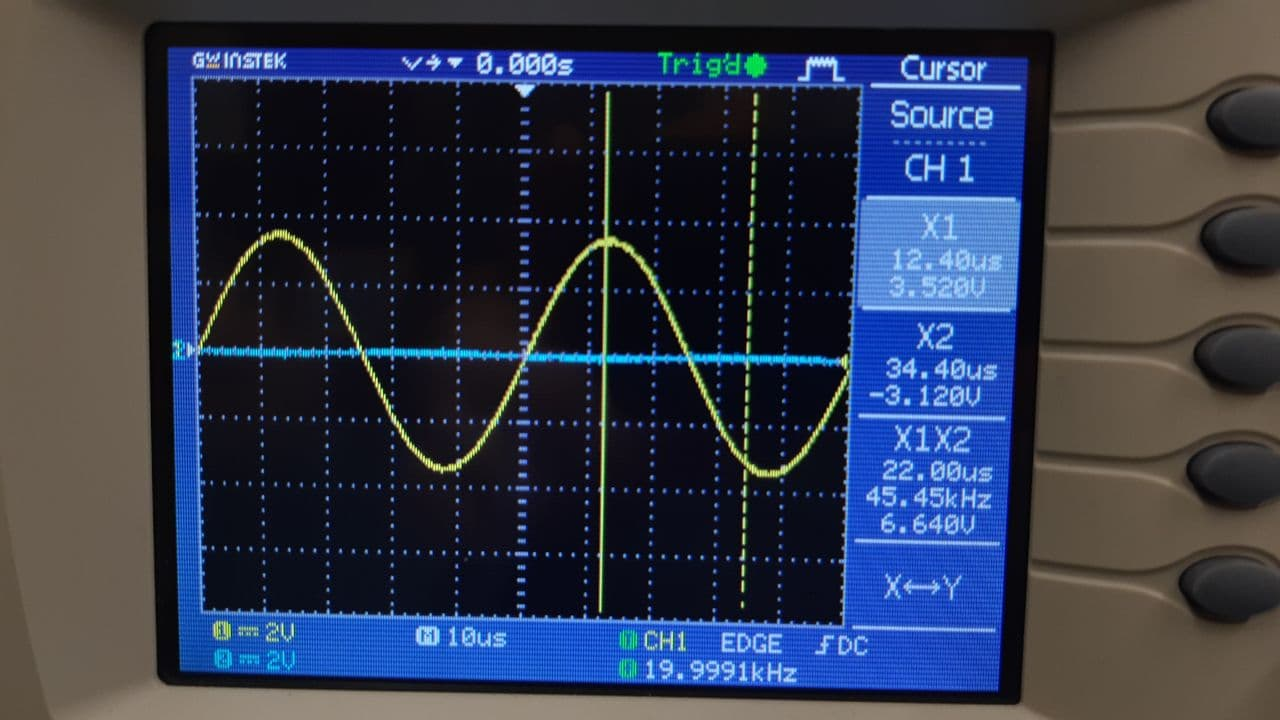
\includegraphics[scale=0.2]{media/f2vc.jpg}
        \caption{$V_C$ f=20kHz}
    \end{figure}

    \FloatBarrier
\subsection{Tabelle}    
\vspace{1cm}        

\begin{table}[!h]
        
            
        \begin{tabular}{|p{2cm}|p{2cm}|p{2cm}|p{2cm}|p{2cm}|p{2cm}|}
            \hline
            \rowcolor{nred} \textit{f}[Hz] & Comp- & $V_{pp}$ [V] & $t_r$ [$\mu$s] & $\varphi$° &  $\varphi$ rad\\
            \hline
            \rowcolor{norange} 500 & R & 3,48 & 300 & 54 & 0,94\\
            \hline
            \rowcolor{norange} 500 & L & 0,4 & 620 & 116,6 & 2,04\\
            \hline
            \rowcolor{norange} 500 & C & 5,84 & -216 & -39 & -0,68\\
            \hline
            \rowcolor{nyellow} \textit{fr} & R & 6,40 & 3 & 5,4 & 0,1\\
            \hline
            \rowcolor{nyellow} \textit{fr} & L & 2,2 & 100 & 83,52 & 1,46\\
            \hline
            \rowcolor{nyellow} \textit{fr} & C & 2,2 & -102  & -85 & 1,5\\
            \hline
            \rowcolor{ngreen}  20k & R & 2,64 & -8,8 & -63,4 & 1,12\\
            \hline
            \rowcolor{ngreen} 20k & L & 6,48 & 2,8 & 20,16 &0,35\\
            \hline
            \rowcolor{ngreen} 20k & C & 0.1 & -12 & -86 & -1,5\\
            \hline
            
        \end{tabular}
        \vskip 0.2cm
        \centering
        \begin{tabular}{|c|c|}
            \hline
            \rowcolor{norange} $R_{pind}$ & $132 \Omega$\\
            \rowcolor{nyellow}  $R_{sperim}$ & $2,16 k\Omega$ \\
            \hline
            
        \end{tabular}
         
    \end{table}
   
    \subsection{Calcoli}
    \begin{center}
        
    \textbf{Calcoli teorici}\\

$fr=\frac{1}{2\pi\cdot\sqrt{LC}}=\frac{1}{2\pi\cdot\sqrt{0,047 H \cdot (100 \cdot 10^{-9})F }}=2,32kHz$\\
\vspace{5mm}
$V_{pp}=7V$\\
$V=\frac{V_{pp}}{2\sqrt{2}}=\frac{V_{pp}}{7\sqrt{2}}=2,47V$\\
\vspace{10mm}
\textit{f=500Hz:}\\

\vspace{5mm}
$X_L=\omega L=2 \pi\cdot f \cdot L=147,8 \Omega=2 \pi\cdot 500Hz \cdot 47mH=147,8 \Omega$\\
$X_C=\frac{1}{\omega \cdot C}=\frac{1}{2 \pi\cdot f  \cdot C}=\frac{1}{2 \pi\cdot 500Hz  \cdot (100 \cdot 10^{-9})F}=3185 \Omega$\\
$Z=\sqrt{R^2+(X_L-X_C)^2}=3038\Omega$\\


\vspace{5mm}
$I=\frac{V}{Z}=\frac{2,47V}{3038\Omega}=0,8mA$\\

\vspace{5mm}

$V_R=R\cdot I=2,2k\Omega \cdot 0,8mA=1,76V$\\
$V_L=X_L\cdot I=147,8 \Omega \cdot 0,8mA=0,12V$\\
$V_C=X_C\cdot I=3185 \Omega\cdot 0,8mA=2,55V$\\
$V=\sqrt{{V_R}^2+(V_L-V_C)^2}=\sqrt{1,76^2+(0,12-2,55)^2}=3V$\\

\vspace{5mm}
$\varphi=\arctan(\frac{X_L - X_C}{R})=\arctan(-1,38)=-54$°\\

\vspace{10mm}
\textit{fr:}\\
\vspace{5mm}
$X_L=\omega L=2 \pi\cdot fr \cdot L=147,8 \Omega=2 \pi\cdot 2,32kHz \cdot 47mH=685 \Omega$\\
$X_C=\frac{1}{\omega \cdot C}=\frac{1}{2 \pi\cdot fr  \cdot C}=\frac{1}{2 \pi\cdot 2,32kHz  \cdot (100 \cdot 10^{-9})F}=686 \Omega$\\
$X_L\simeq X_C$\\
$Z=\sqrt{R^2+(X_L-X_C)^2}=R=2,2 k\Omega$\\


\vspace{5mm}
$I=\frac{V}{Z}=\frac{V}{R}=\frac{2,47V}{2,2k\Omega}=1,2mA$\\

\vspace{5mm}

$V_R=R\cdot I=2,2k\Omega \cdot 1,2mA=2,64v$\\
$V_L=X_L\cdot I=685 \Omega \cdot 1,2mA=0,77V$\\
$V_C=X_C\cdot I=686 \Omega\cdot 1,2mA=0,82V$\\
$V=\sqrt{{V_R}^2+(V_L-V_C)^2}=\sqrt{2,64^2+(0,77-0,82)^2}=2,64V$\\
\vspace{5mm}
$\varphi=\arctan(\frac{X_L - X_C}{R})= \arctan (\frac{1}{2200})=0,026$°\\ 
\vspace{10mm}
\textit{f=20kHz}\\
\vspace{5mm}
$X_L=\omega L=2 \pi\cdot f \cdot L=147,8 \Omega=2 \pi\cdot 20kHz \cdot 47mH=5,9 k\Omega$\\
$X_C=\frac{1}{\omega \cdot C}=\frac{1}{2 \pi\cdot f  \cdot C}=\frac{1}{2 \pi\cdot 20kHz  \cdot (100 \cdot 10^{-9})F}=80 \Omega$\\
$Z=\sqrt{R^2+(X_L-X_C)^2}=6621\Omega$\\


\vspace{5mm}
$I=\frac{V}{Z}=\frac{2,47V}{6621\Omega}=0,04mA$\\

\vspace{5mm}

$V_R=R\cdot I=2,2k\Omega \cdot 0,04mA=0.88V$\\
$V_L=X_L\cdot I=5,9 k\Omega \cdot 0,04mA=2,36V$\\
$V_C=X_C\cdot I= 80\Omega\cdot 0,04mA=0,03V$\\
$V=\sqrt{{V_R}^2+(V_L-V_C)^2}=\sqrt{0,88^2+(2,36-0,03)^2}=2,49V$\\

\vspace{5mm}
$\varphi=\arctan(\frac{X_L - X_C}{R})=\arctan(2,64)=69,3$°\\
\vspace{10mm}
\textbf{Calcoli con valori sperimentali}\\
\vspace{5mm}
f=500Hz\\
\vspace{5mm}
$V_R=\frac{V_{PPR}}{2\sqrt{2}}=\frac{3,48}{2\sqrt{2}}=1,23V$\\
$V_L=\frac{V_{PPL}}{2\sqrt{2}}=\frac{0,4}{2\sqrt{2}}=0,14V$\\
$V_C=\frac{V_{PPC}}{2\sqrt{2}}=\frac{5,84}{2\sqrt{2}}=2,06V$\\
$V=\sqrt{{V_R}^2+(V_L-V_C)^2}=\sqrt{{1,23}^2+(0,14-2,06)^2}=2,28V$\\
\vspace{5mm}
formule generali:\\
${\varphi}:2\pi=t:T$ \\
${\varphi}=\frac{2\pi \cdot t}{T}$\\
${\varphi}rad:2\pi=x:360$\\
$\varphi$°=$\frac{\varphi rad \cdot 360}{2\pi}$\\
\vspace{10mm}

${\varphi}_R=\frac{2\pi \cdot t_R}{T}=\frac{2\pi \cdot (300 \cdot 10^{-6})s}{1/500Hz}=1$rad\\
${\varphi}_R$°=$\frac{\varphi rad \cdot 360}{2\pi}=\frac{1 \cdot 360}{2\pi}$=57°\\
\vspace{5mm}

${\varphi}_L=\frac{2\pi \cdot t_L}{T}=\frac{2\pi \cdot (620 \cdot 10^{-6})s}{1/500Hz}=1,94$rad\\
${\varphi}_L$°=$\frac{\varphi rad \cdot 360}{2\pi}=\frac{1,94 \cdot 360}{2\pi}$=111°\\
\vspace{5mm}

${\varphi}_C=\frac{2\pi \cdot t_C}{T}=\frac{2\pi \cdot (-216 \cdot 10^{-6})s}{1/500Hz}=-0,67$rad\\
${\varphi}_C$°=$\frac{\varphi rad \cdot 360}{2\pi}=\frac{-0,67 \cdot 360}{2\pi}$=-38°\\

\vspace{10mm}
fr=2,32kHz\\
\vspace{5mm}
$V_R=\frac{V_{PPR}}{2\sqrt{2}}=\frac{6,4}{2\sqrt{2}}=2,26V$\\
$V_L=\frac{V_{PPL}}{2\sqrt{2}}=\frac{2,2}{2\sqrt{2}}=0,78V$\\
$V_C=\frac{V_{PPC}}{2\sqrt{2}}=\frac{2,2}{2\sqrt{2}}=0,78V$\\
$V=V_R=2,26V$\\
\vspace{5mm}
formule generali:\\
${\varphi}:2\pi=t:T$ \\
${\varphi}=\frac{2\pi \cdot t}{T}$\\
${\varphi}rad:2\pi=x:360$\\
$\varphi$°=$\frac{\varphi rad \cdot 360}{2\pi}$\\
\vspace{10mm}

${\varphi}_R=\frac{2\pi \cdot t_R}{T}=\frac{2\pi \cdot (3 \cdot 10^{-6})s}{1/2320}=0,044$rad\\
${\varphi}_R$°=$\frac{\varphi rad \cdot 360}{2\pi}=\frac{0,44 \cdot 360}{2\pi}$=2,5°\\
\vspace{5mm}

${\varphi}_L=\frac{2\pi \cdot t_L}{T}=\frac{2\pi \cdot (100 \cdot 10^{-6})s}{1/2320Hz}=1,45$rad\\
${\varphi}_L$°=$\frac{\varphi rad \cdot 360}{2\pi}=\frac{1,45 \cdot 360}{2\pi}$=83°\\
\vspace{5mm}

${\varphi}_C=\frac{2\pi \cdot t_C}{T}=\frac{2\pi \cdot (-102 \cdot 10^{-6})s}{1/2320Hz}=-1,48$rad\\
${\varphi}_C$°=$\frac{\varphi rad \cdot 360}{2\pi}=\frac{-1,48 \cdot 360}{2\pi}$=-85°\\

\vspace{10mm}
f=20kHz\\
\vspace{5mm}
$V_R=\frac{V_{PPR}}{2\sqrt{2}}=\frac{2,64}{2\sqrt{2}}=0,9V$\\
$V_L=\frac{V_{PPL}}{2\sqrt{2}}=\frac{6,48}{2\sqrt{2}}=2,29V$\\
$V_C=\frac{V_{PPC}}{2\sqrt{2}}=\frac{0,1}{2\sqrt{2}}=0,03V$\\
$V=\sqrt{{V_R}^2+(V_L-V_C)^2}=\sqrt{{0,9}^2+(2,29-0,03)^2}=2,4V$\\
\vspace{5mm}
formule generali:\\
${\varphi}:2\pi=t:T$ \\
${\varphi}=\frac{2\pi \cdot t}{T}$\\
${\varphi}rad:2\pi=x:360$\\
$\varphi$°=$\frac{\varphi rad \cdot 360}{2\pi}$\\
\vspace{10mm}

${\varphi}_R=\frac{2\pi \cdot t_R}{T}=\frac{2\pi \cdot (-8,8 \cdot 10^{-6})s}{1/20kHz}=-1,1$rad\\
${\varphi}_R$°=$\frac{\varphi rad \cdot 360}{2\pi}=\frac{-1,1 \cdot 360}{2\pi}$=63,4°\\
\vspace{5mm}

${\varphi}_L=\frac{2\pi \cdot t_L}{T}=\frac{2\pi \cdot (2,8 \cdot 10^{-6})s}{1/20kHz}=0,35$rad\\
${\varphi}_L$°=$\frac{\varphi rad \cdot 360}{2\pi}=\frac{1,94 \cdot 360}{2\pi}$=20,2°\\
\vspace{5mm}

${\varphi}_C=\frac{2\pi \cdot t_C}{T}=\frac{2\pi \cdot (-12 \cdot 10^{-6})s}{1/20kHz}=-1,5$rad\\
${\varphi}_C$°=$\frac{\varphi rad \cdot 360}{2\pi}=\frac{-0,67 \cdot 360}{2\pi}$=-86,4°\\

\vspace{10mm}
\vspace{5mm}
\end{center}



\section{Conclusioni}
Osservando i risultati ottenuti possiamo notare che viene seguito il comportamento teorico del circuito a parte per lo sfasamento dato
dalla resistenza parassita dell'induttore che risulta rilevante solo quando vengono paragonati i valori teorici e quelli misurati, per quanto riguarda i 
diagrammi vettoriali esso non presenta un problema. 
Lo sfasamento pratico della tensione sulla corrente è uguale a $\varphi$ di R perchè la tensione ai capi di R è in fase con la corrente
e dal momento che per comodità abbiamo stabilito che $\vec{V}$ è posizionato sull'asse delle X.\\
Avendo eseguito i calcoli possiamo comparare i valori teorici con quelli pratici e calcolarne la discrepanza:\\
\begin{center}
    \begin{table}[!h]
        
    
    \begin{tabular}{|c|c|c|c|c|c|}
     \hline
       \rowcolor{nred} freq &  & val. teo & val sper. & disc. \%\\ \hline
       
      \multirow{5}{*}{500Hz} &\cellcolor{norange} $V_R$ & \cellcolor{norange}1, 76V& \cellcolor{norange}1,23&\cellcolor{norange} 30\\ \cline{2-5}
      
                            & \cellcolor{norange}$V_L$ &\cellcolor{norange} 0,12 V&\cellcolor{norange} 0,14V &\cellcolor{norange}16 \\ \cline{2-5}

                            & \cellcolor{norange}$V_C$ &\cellcolor{norange}2,55 V&\cellcolor{norange} 2,06V& \cellcolor{norange}20\\\cline{2-5}
     
                            &\cellcolor{norange} $V$   &\cellcolor{norange} 3V&\cellcolor{norange} 2,28V& \cellcolor{norange}24 \\\cline{2-5}

                            &\cellcolor{norange} $\varphi$ &\cellcolor{norange}54° & \cellcolor{norange}57°& \cellcolor{norange}5 \\\hline
    
                            \multirow{5}{*}{2,32kHz} &\cellcolor{nyellow} $V_R$ &\cellcolor{nyellow} 2,64V& \cellcolor{nyellow}2,26V& \cellcolor{nyellow}14\\\cline{2-5}
      
                            &\cellcolor{nyellow} $V_L$ &\cellcolor{nyellow} 0,77V& \cellcolor{nyellow}0,78V &\cellcolor{nyellow}1,2 \\\cline{2-5}
    
                            &\cellcolor{nyellow} $V_C$ &\cellcolor{nyellow}0,82V&\cellcolor{nyellow} 0,78V&\cellcolor{nyellow} 5\\\cline{2-5}
    
                            &\cellcolor{nyellow} $V$   &\cellcolor{nyellow} 2,64V&\cellcolor{nyellow} 2,26V&\cellcolor{nyellow} 14 \\\cline{2-5}
    
                            & \cellcolor{nyellow}$\varphi$ &\cellcolor{nyellow}0,026° &\cellcolor{nyellow} 2,5°& \cellcolor{nyellow}1000\\\hline
    
   
                            \multirow{5}{*}{20kHz} & \cellcolor{ngreen}$V_R$ &\cellcolor{ngreen} 0,88V&\cellcolor{ngreen} 0,9V&\cellcolor{ngreen}2 \\\cline{2-5}
      
                            & \cellcolor{ngreen}$V_L$ &\cellcolor{ngreen} 2,36V&\cellcolor{ngreen} 2,29V &\cellcolor{ngreen} 3\\\cline{2-5}
    
                            &\cellcolor{ngreen} $V_C$ &\cellcolor{ngreen}0,03V&\cellcolor{ngreen} 0,03V&\cellcolor{ngreen}0\\\cline{2-5}
    
                            &\cellcolor{ngreen} $V$   &\cellcolor{ngreen} 2,49V& \cellcolor{ngreen}2,4V&\cellcolor{ngreen} 3,61\\\cline{2-5}
    
                            & \cellcolor{ngreen}$\varphi$ &\cellcolor{ngreen}69,3° &\cellcolor{ngreen} 63,4°& \cellcolor{ngreen}8 \\\hline
                           

    \end{tabular}
\end{table}
$Discrepanza \%=\frac{Val. teo.-Val. sper.}{Val. teo.}\cdot 100$
\end{center}
\FloatBarrier 
$Discrepanza=\frac{Val. teo.-Val. sper.}{Val. teo.}\cdot 100$
\vspace{2mm}

Possiamo notare osservando la discrepanza che gli i valori pratici e teorici alla frequenza di 500Hz sono mediamente pù distanti tra loro 
, questo perchè a quella frequenza si nota maggiormente la resistenza parassita dell'induttore che va a influire sulle tensioni sperimentali infatti possiamo 
calcolare la caduta di tensione provocata tramite la legge di Ohm $V_{rp}=I\cdot R_{pind}=0,8mA \cdot 132 \Omega=0.11V$, inoltre questa resistenza parassita va a influire anche sugli sfasamenti
infatti con la formula\\ 
\begin{center}
$\varphi_L=\arccos(\frac{V_{Lteo}}{V_{Lsper}})$ = $\arccos(\frac{0,12V}{0,14V})$ = 30°\\
    
\end{center}
$\varphi_L=\arccos(\frac{V_{Lteo}}{V_{Lsper}})$ = $\arccos(\frac{0,12V}{0,14V})$ = 30°\\
si va a ricavare lo sfasamento provocato da questo fenomeno ($\varphi_L$) che si andrà ad aggiungere allo sfasamento totale ($\varphi$) usando la formula $\varphi_{tot}=\varphi+90-\varphi_L$, nel nostro caso lo sfasamento totale risulta 98°.\\
L'ultimo punto da chiarire è la discrepanza di $\varphi$ nella frequenza di risonanza, risulta altissima perchè lo sfasamento dovrebbe essere di 0° mentre 
a causa degli errori sistematici e gli errori accumulati dai vari strumenti da 0° sperimentalmente ne risulta 2,5° che è comunque accettabile ma visto che il valore teorico è cosi basso la discrepanza risulta sfalsata.\\
$\varphi_R$ a 500Hz calcolato teoricamente risulta negativo perchè con quel metodo si considera lo sfasamento della tensione rispetto alla corrente mentre sperimentalmente abbiamo fatto il contrario ossia abbiamo considerato lo sfasamento della corrente rispetto 
alla tensione.\\
\subsection{Diagrammi vettoriali}
u=1V ma sono stati usati nel grafico i valori picco picco.\\
\textit{f=500Hz}   u=1V \\
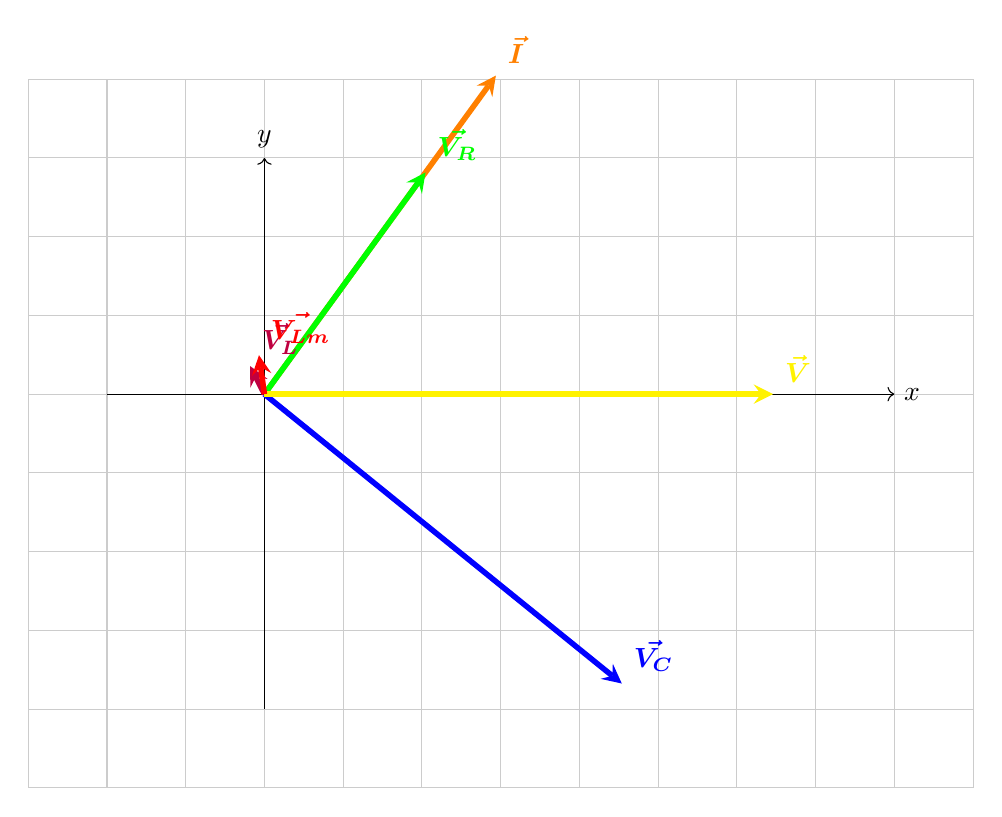
\begin{tikzpicture}
    \draw[thin,gray!40] (-3,-5) grid (9,4);
    \draw[->] (-2,0)--(8,0) node[right]{$x$};
    \draw[->] (0,-4)--(0,3) node[above]{$y$};
    \draw[line width=2pt,orange,-stealth] (0,0) -- (54:5cm) node[anchor=south west]{$\boldsymbol{\vec{I}}$};
    \draw[line width=2pt,green,-stealth] (0,0) -- (54:3.48cm) node[anchor=south west]{$\boldsymbol{\vec{V_R}}$};
    \draw[line width=2pt,blue,-stealth] (0,0) -- (-39:5.84cm) node[anchor=south west]{$\boldsymbol{\vec{V_C}}$};
    \draw[line width=2pt,purple,-stealth] (0,0) -- (117:0.4cm) node[anchor=south west]{$\boldsymbol{\vec{V_L}}$};
    \draw[line width=2pt,yellow,-stealth] (0,0) -- (0:6.46cm) node[anchor=south west]{$\boldsymbol{\vec{V}}$};
    \draw[line width=2pt,red,-stealth] (0,0) -- (98:0.5cm) node[anchor=south west]{$\boldsymbol{\vec{V_{Lm}}}$};
    
      

  \end{tikzpicture}

  \vskip 3cm

 


  \textit{fr}\\
  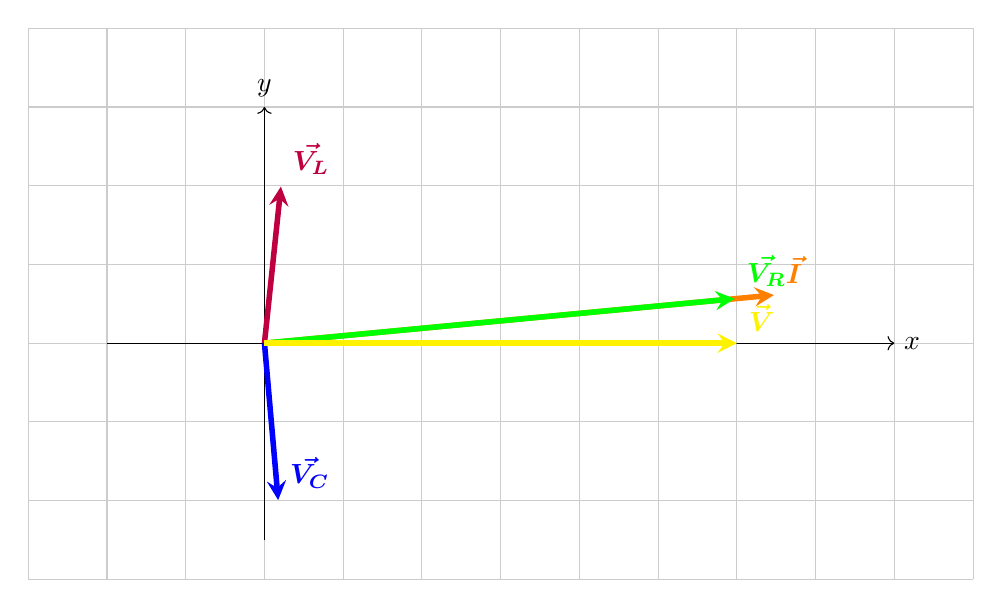
\begin{tikzpicture}
    \draw[thin,gray!40] (-3,-3) grid (9,4);
    \draw[->] (-2,0)--(8,0) node[right]{$x$};
    \draw[->] (0,-2.5)--(0,3) node[above]{$y$};
    \draw[line width=2pt,orange,-stealth] (0,0) -- (5.4:6.5cm) node[anchor=south west]{$\boldsymbol{\vec{I}}$};
    \draw[line width=2pt,green,-stealth] (0,0) -- (5.4:6cm) node[anchor=south west]{$\boldsymbol{\vec{V_R}}$};
    \draw[line width=2pt,blue,-stealth] (0,0) -- (-85:2cm) node[anchor=south west]{$\boldsymbol{\vec{V_C}}$};
    \draw[line width=2pt,purple,-stealth] (0,0) -- (84:2cm) node[anchor=south west]{$\boldsymbol{\vec{V_L}}$};
    \draw[line width=2pt,yellow,-stealth] (0,0) -- (0:6cm) node[anchor=south west]{$\boldsymbol{\vec{V}}$};
   
 
  \end{tikzpicture}
\vskip 1cm
  
  \textit{f=20kHz}\\
  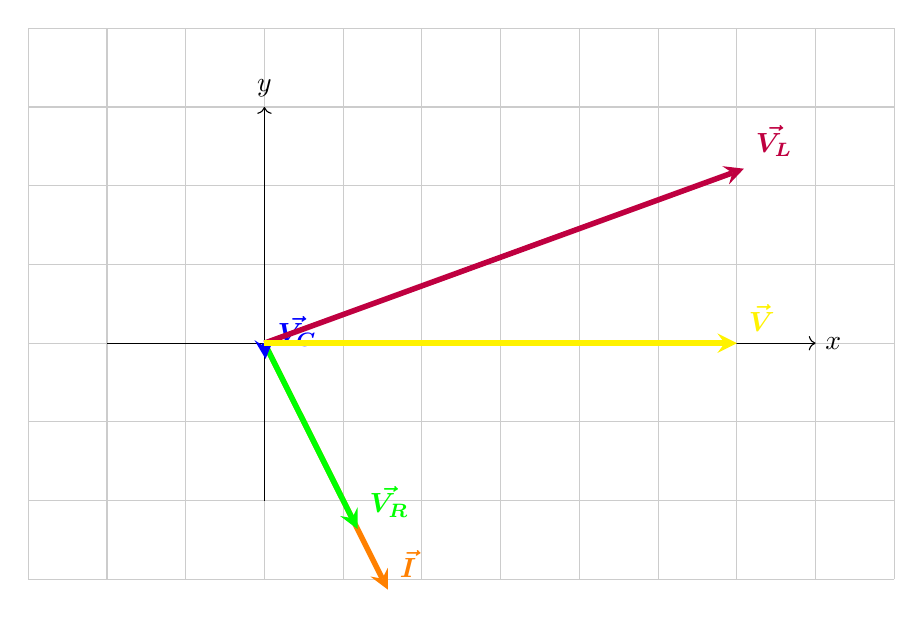
\begin{tikzpicture}
    \draw[thin,gray!40] (-3,-3) grid (8,4);
    \draw[->] (-2,0)--(7,0) node[right]{$x$};
    \draw[->] (0,-2)--(0,3) node[above]{$y$};
    \draw[line width=2pt,orange,-stealth] (0,0) -- (-63.4:3.5cm) node[anchor=south west]{$\boldsymbol{\vec{I}}$};
    \draw[line width=2pt,green,-stealth] (0,0) -- (-63.4:2.64cm) node[anchor=south west]{$\boldsymbol{\vec{V_R}}$};
    \draw[line width=2pt,blue,-stealth] (0,0) -- (-86:0.2cm) node[anchor=south west]{$\boldsymbol{\vec{V_C}}$};
    \draw[line width=2pt,purple,-stealth] (0,0) -- (20:6.48cm) node[anchor=south west]{$\boldsymbol{\vec{V_L}}$};
    \draw[line width=2pt,yellow,-stealth] (0,0) -- (0:6cm) node[anchor=south west]{$\boldsymbol{\vec{V}}$};
      
  \end{tikzpicture}
  
\end{document}
